\documentclass[xcolor=x11names]{beamer}
  \mode<presentation> {
    \usetheme{Frankfurt}
  }

\usepackage{times}
\usepackage{amsmath,amssymb}
\usepackage[english]{babel}
\usepackage[utf8]{inputenc}
% \usepackage[latin1]{inputenc}
\usepackage{array}
% % !BIB TS-program = biber
% !BIB program = biber
%===============================================================================
%          File: preamble.tex
%        Author: Pedro Ferrari
%       Created: 08 Feb 2017
% Last Modified: 08 Feb 2017
%   Description: Preamble for Thesis File
%===============================================================================
%---------------------------------------+
% Source code, programming and patching |
%---------------------------------------+
\usepackage{etoolbox}    % Toolbox of programming tools
\usepackage{xpatch}      % Extension of etoolbox patching commands

%--------------------------------------+
% Language, hyphenation, encoding, etc |
%--------------------------------------+
\usepackage[english]{babel}
\usepackage{lmodern}             % Use Latin Modern fonts
\usepackage[T1]{fontenc}         % Better output when a diacritic/accent is used
\usepackage[utf8]{inputenc}      % Allows to input accented characters
\usepackage{textcomp}            % Avoid conflicts with siunitx and microtype
\usepackage{microtype}           % Improves justification and typography
\usepackage[svgnames]{xcolor}    % Svgnames option loads navy (blue) colour

%---------------------------------------------+
% Page style: titles, margins, footnotes, etc |
%---------------------------------------------+
% A4 page layout:
\usepackage[width=14cm,left=3.5cm,marginparwidth=3cm,marginparsep=0.35cm,
height=21cm,top=3.7cm,headsep=1cm,footskip=1.1cm]{geometry}

\usepackage[pagestyles,outermarks]{titlesec}  % Customize titles and headers
\newpagestyle{main}[\scshape]{%
  \headrule
  \sethead
  [\thepage][][\chaptertitlename\space\thechapter. \chaptertitle]
  {\ifthesection{\thesection\space\,\sectiontitle}
  {\chaptertitlename\space\thechapter. \chaptertitle}}{}{\thepage}
}
\newpagestyle{special}[\scshape]{%
  \headrule
  \sethead
  [\thepage][][\chaptertitle]
  {\ifthesection{\sectiontitle}{\chaptertitle}}{}{\thepage}
}
% The following pagestyle is needed because titlesec isn't compatible with
% refsegment=chapter
\newpagestyle{bibatend}[\scshape]{
  \headrule
  \sethead
  [\thepage][][\chaptertitle]
  {\sectiontitle}{}{\thepage}
}
\pagestyle{special}
\appto{\mainmatter}{\pagestyle{main}}
\appto{\backmatter}{\pagestyle{bibatend}}
\appto{\printindex}{\pagestyle{special}}

% Use empty page style instead of plain in parts and chapters title pages
\patchcmd{\part}{plain}{empty}{}{}
\patchcmd{\chapter}{plain}{empty}{}{}

\usepackage{emptypage}  % Empty blank pages created by \cleardoublepage

% Change chapter heading style to match titlepage
\titleformat{\chapter}[display]
{\bfseries\filcenter}
{\titlerule[1.5pt]\vspace{4ex}%
\LARGE{\chaptertitlename\space\thechapter}}{0.5cm}{\huge}
[\vspace{2ex}{\titlerule[1.5pt]}\vspace{0.3cm}]
% Do the same for unnumbered chapters (TOC, preface, etc)
\titleformat{name=\chapter,numberless}[display]
{\bfseries\filcenter}
{\titlerule[1.5pt]\vspace{4ex}}{0.5cm}{\huge}
[\vspace{2ex}{\titlerule[1.5pt]}\vspace{0.3cm}]

\usepackage[stable,multiple]{footmisc}  % Customizations of footnotes
\renewcommand*{\footnoterule}{\vspace*{0.3cm}\hrule width 2.5cm\vspace*{0.3cm}}
\makeatletter
  \renewcommand\@makefntext[1]{
  \setlength{\parindent}{15pt}\mbox{\@thefnmark.\space}{#1}}
\makeatother

%-------------------------------+
% Math symbols and environments |
%-------------------------------+
\usepackage{amsmath}               % Load new math environments
\numberwithin{equation}{section}
\usepackage{amssymb}               % Defines most math symbols (such as \mathbb)
\usepackage{mathtools}             % Extension and bug fixes for amsmath package
\usepackage{mathrsfs}              % Math script like font
\usepackage{breqn}                 % Automatic line breaking of math expressions
\renewcommand*{\intlimits}{\displaylimits}  % Fix breqn clash with intlimits


%---------------------+
% Floats and captions |
%---------------------+
\usepackage{graphicx}           % To include graphics files
%\graphicspath{{/Users/Pedro/OneDrive/programming/Latex/logos/}{figures/}{tables/}}
\usepackage{pdflscape}
\usepackage[font=small,labelfont=bf]{caption}
\captionsetup*[figure]{format=plain,justification=centerlast,labelsep=quad}
\captionsetup*[table]{justification=centering,labelsep=newline}
\numberwithin{figure}{section}
\numberwithin{table}{section}

% Use subcaption for subfigures (to work properly with hyperref)
\usepackage{subcaption}
\captionsetup*[subfigure]{subrefformat=simple,labelformat=simple}
\renewcommand*{\thesubfigure}{(\alph{subfigure})}

% Further modifications of float layout
\usepackage[captionskip=5pt]{floatrow}  % We set caption skip here
\floatsetup[table]{style=Plaintop,font=small,footnoterule=none,footskip=2.5pt}

%----------------+
% Table packages |
%----------------+
\usepackage{array}          % Flexible column formatting
% \usepackage{spreadtab}  % Spreadsheet features
\usepackage{multirow}       % Allows table cells that span more than one row
\usepackage{booktabs}       % Enhance quality of tables
\setlength{\heavyrulewidth}{1pt}

% \usepackage{longtable}        % Allows to break tables through pages
% \floatsetup[longtable]{margins=centering,LTcapwidth=table}


%---------------------------------------------------------+
% Miscellaneous packages: lists, setspace, todonotes, etc |
%---------------------------------------------------------+
\usepackage[shortlabels,inline]{enumitem}   % Customize lists
\setlist[itemize,1]{label=$\bullet$}
\setlist[itemize,2]{label=\footnotesize{$\blacktriangleright$}}
\setlist[itemize,3]{label=\tiny{$\blacksquare$}}
\setlist[itemize,4]{label=\bfseries{\large{--}}}
% \setlist[enumerate,2]{label=\emph{\alph*})}
\newlist{steps}{enumerate}{1}               % List of steps to be used in proofs
\setlist[steps,1]{leftmargin=*,label=\textit{Step \arabic*.},ref=\arabic*}

\usepackage{setspace}  % Commands for double and one-and-a-half spacing
\setstretch{1.2}       % 1.2 spacing

% \usepackage{listings}  % Useful for inserting code (no unicode support)
% \lstset{basicstyle=\small\ttfamily}

% \usepackage[colorinlistoftodos,textsize=small,figheight=5cm,
% figwidth=10cm,color=red!85]{todonotes}

% \usepackage{lipsum}    % Dummy text generator

\usepackage{algorithm2e} % to write pseudo-code algorithms
\usepackage{qtree} % To draw trees
\usepackage{todonotes} % To draw trees

%----------------------------------+
% Appendix, bibliography and index |
%----------------------------------+
% Solve bad interaction between titlesec and \appendix
\preto{\appendix}{\cleardoublepage}

% this might insert blank pages here and there but now compilation works correctly with biber
\usepackage[style=american]{csquotes}  % Language sensitive quotation facilities
\usepackage[style=authoryear-comp,backref=true,refsection=chapter,backend=biber]{biblatex}

% \usepackage[
% 	backend=biber,
% 	sortlocale=us_EN,
% 	natbib=true,
% 	style=authoryear-comp,backref=true,refsection=chapter,
% 	url=false,
% 	doi=true,
% 	eprint=false
% 	]{biblatex}

\addbibresource{biblio.bib}

% Bibliography format
\usepackage{mybibformat} % Modifications to authoryear-comp style and hyperlinks
\setlength{\bibitemsep}{0.1cm}

\usepackage{imakeidx}  % Creation and formatting of indexes
\indexsetup{level=\chapter,firstpagestyle=empty,othercode=\small}
\makeindex[title=Alphabetical Index]

%------------------------------------------------------+
% Hyperlinks, bookmarks, theorems and cross-references |
%------------------------------------------------------+
\usepackage[hyperfootnotes=false]{hyperref}
\hypersetup{colorlinks=true, allcolors=Navy, linktoc=page,
pdfstartview={XYZ null null 1}, pdfcreator={Vim LaTeX},
pdfsubject={Machine Learning},
pdftitle={Math thesis},
pdfauthor={Juan Mateo De Monasterio},
pdfkeywords={machine learning}
}
\usepackage[numbered,open,openlevel=1]{bookmark}

\usepackage{amsthm,amsmath}        % We load theorem environments here to avoid warnings

\usepackage[noabbrev,capitalise]{cleveref}

%-----------------------------------------------------------+
% Comment out the math equations, figurest,etc                |
% This will help us spell checking the doc with online tools |
%-----------------------------------------------------------+

% These allow one to compile the pdf without any figures, equations
% etc. which will let us copy paste the output for spell checking.

%\usepackage{comment}
%\excludecomment{figure}
%\let\endfigure\relax
%\excludecomment{equation}
%\let\endequation\relax

%\excludecomment{lstlisting}
%\let\endlstlisting\relax



%------------------------------------+
% Definition of theorem environments |
%------------------------------------+
% Declare theorem styles that remove final dot and use bold font for notes
\newtheoremstyle{plaindotless}{\topsep}{\topsep}{\itshape}{0pt}{\bfseries}{}%
{5pt plus 1pt minus 1pt}{\thmname{#1}\thmnumber{ #2}\bfseries{\thmnote{ (#3)}}}
\newtheoremstyle{definitiondotless}{\topsep}{\topsep}{\normalfont}{0pt}%
{\bfseries}{}{5pt plus 1pt minus 1pt}%
{\thmname{#1}\thmnumber{ #2}\bfseries{\thmnote{ (#3)}}}
\newtheoremstyle{remarkdotless}{0.5\topsep}{0.5\topsep}{\normalfont}{0pt}%
{\itshape}{}{5pt plus 1pt minus 1pt}%
{\thmname{#1}\normalfont\thmnumber{ #2}\itshape{\thmnote{ (#3)}}}

% Define style dependent environments and number them consecutively per section
\theoremstyle{plaindotless}
\newtheorem{theorem}{Theorem}[section]
\newtheorem*{theorem*}{Theorem.}
\newtheorem{proposition}[theorem]{Proposition}
\newtheorem*{proposition*}{Proposition.}
\newtheorem{lemma}[theorem]{Lemma}
\newtheorem*{lemma*}{Lemma.}
\newtheorem{corollary}[theorem]{Corollary}
\newtheorem*{corollary*}{Corollary.}

\theoremstyle{definitiondotless}
\newtheorem{definition}[theorem]{Definition}
\newtheorem*{definition*}{Definition.}
\newtheorem{examplex}[theorem]{Example}
\newtheorem*{examplestarred}{Example.}
\newtheorem*{continuedex}{Example \continuedexref\space Continued.}
\newtheorem{exercise}[theorem]{Exercise}
\newtheorem*{exercise*}{Exercise.}
\newtheorem*{solution*}{Solution.}
\newtheorem{problem}{Problem}

\theoremstyle{remarkdotless}
\newtheorem{remark}[theorem]{Remark}
\newtheorem*{remark*}{Remark.}
\newtheorem*{notation*}{Notation.}

% Define numbered, unnumbered and continued examples with triangle end mark
\newcommand{\myqedsymbol}{\ensuremath{\triangle}}

\newenvironment{example}
  {\pushQED{\qed} \renewcommand{\qedsymbol}{\myqedsymbol}\examplex}
  {\popQED\endexamplex}

\newenvironment{example*}
  {\pushQED{\qed}\renewcommand{\qedsymbol}{\myqedsymbol}\examplestarred}
  {\popQED\endexamplestarred}

\newenvironment{examcont}[1]
  {\pushQED{\qed}\renewcommand{\qedsymbol}{\myqedsymbol}%
    \newcommand{\continuedexref}{\ref*{#1}}\continuedex}
  {\popQED\endcontinuedex}


%-----------------------------------------------+
% Cross-references settings (cleveref settings) |
%-----------------------------------------------+

\crefname{exercise}{Exercise}{Exercises}
\crefname{enumerate}{Enumeration}{Enumerations}
\crefname{stepsi}{Step}{Steps}
\crefname{problem}{Problem}{Problems}

\crefname{equation}{}{}
\crefformat{equation}{#2(#1)#3}
\crefrangeformat{equation}{#3(#1)#4 to #5(#2)#6}
\crefmultiformat{equation}{#2(#1)#3}{ and #2(#1)#3}{, #2(#1)#3}{ and #2(#1)#3}
\crefrangemultiformat{equation}{#3(#1)#4 to #5(#2)#6}{ and #3(#1)#4 to #5(#2)#6}%
{, #3(#1)#4 to #5(#2)#6}{ and #3(#1)#4 to #5(#2)#6}

%----------------------------------------------+
% Half-title, titlepage and copyright settings |
%----------------------------------------------+

\newcommand*{\halftitlepg}{%
  \begingroup
    \begin{center}
      \textbf{\huge{Math Thesis}}
    \end{center}
  \endgroup
  \thispagestyle{empty}\cleardoublepage
}

\newcommand*{\titlepg}{%
  \begingroup
    \vspace{0.01\textheight}
    \begin{center}
      \textbf{\LARGE{Universidad de Buenos Aires}}\\
      \vspace{0.02\textheight}
      \textbf{\Large{Facultad de Ciencias Exactas}}\\
      \vspace{0.3\textheight}
      \rule{\textwidth}{1.5pt}\par
      \vspace{\baselineskip}
 {\bfseries\Huge{Explorando migraciones chagásicas en latinoamérica con aprendizaje automático}\par
 	\bigskip\Large{Exploring Latino American chagasic migrations with machine learning}}\\
      \vspace{\baselineskip}
      \rule{\textwidth}{1.5pt}\par
      \vfill
      \textsc{\huge{Juan Mateo De Monasterio}}
      \vfill
      \textbf{\Large{\today}}
    \end{center}
  \endgroup
  \thispagestyle{empty}\clearpage
}

\newcommand*{\copyrightpg}{%
  \begingroup
    \footnotesize
    \parindent 0pt
    \null
    \vfill
    \textcopyright{} 2017 Juan Mateo De Monasterio. All rights reserved.\par
    \vspace{\baselineskip}
    This document is free; you can redistribute it and/or modify it under the
    terms of the GNU General Public License as published by the Free Software
    Foundation; either version 2 of the License, or (at your choice) any later
    version.\par
    \vspace{\baselineskip}
    This document was typeset in Latin Modern font using \LaTeX.\par
  \endgroup
  \thispagestyle{empty}\clearpage
}

\newcommand*{\dedication}{%
  \begingroup
    \vspace*{0.3\textheight}
    \begin{center}
      \emph{\large{To all.}}
      \end{center}
    \endgroup
  \thispagestyle{empty}\cleardoublepage
}

%-------------------+
% Table of contents |
%-------------------+
% Add bookmark for table of contents and increase spacing of items
\preto{\tableofcontents}{\cleardoublepage\pdfbookmark[0]{\contentsname}{toc}%
  \setstretch{1.1}}
\appto{\tableofcontents}{\singlespacing}

%---------------------------------------------------+
% (Re)Definition of new commands and math operators |
%---------------------------------------------------+
% Numbers
\DeclareMathOperator{\N}{\mathbb{N}}
\DeclareMathOperator{\Z}{\mathbb{Z}}
\DeclareMathOperator{\Q}{\mathbb{Q}}
\DeclareMathOperator{\R}{\mathbb{R}}
% Probability
\DeclareMathOperator{\E}{\mathbb{E}}
\DeclareMathOperator{\Expect}{\mathbb{E}}
\DeclareMathOperator{\Var}{\mathrm{Var}}
\DeclareMathOperator{\Cov}{\mathrm{Cov}}
% Delimiters
\DeclarePairedDelimiter{\abs}{\lvert}{\rvert}
\DeclarePairedDelimiter{\norm}{\lvert\lvert}{\rvert\rvert}
% Miscellaneous
\renewcommand{\d}{\ensuremath{\operatorname{d}\!}}  % Differential
\renewcommand{\L}{\ensuremath{\operatorname{\mathcal{L}}}}  % Lagrangian
\DeclareMathOperator{\calN}{\mathcal{N}}
\DeclareMathOperator{\calG}{\mathcal{G}}
\DeclareMathOperator{\calL}{\mathcal{L}}
\DeclareMathOperator{\calE}{\mathcal{E}}
% argmin and max operators
\DeclareMathOperator*{\argmin}{argmin} % no space, limits underneath in displays
% \DeclareMathOperator{\argmin}{argmin} % no space, limits on side in displays
\DeclareMathOperator*{\argmax}{argmax} % no space, limits underneath in displays
% \DeclareMathOperator{\argmax}{argmax} % no space, limits on side in displays



\newcommand\MyBox[2]{
	\fbox{\lower0.75cm
		\vbox to 1.7cm{\vfil
			\hbox to 1.7cm{\hfil\parbox{1.4cm}{#1\\#2}\hfil}
			\vfil}%
	}%
}



\usepackage{fancybox}
\usefonttheme[onlymath]{serif}
\boldmath

\usepackage{scalefnt}
\usepackage{ragged2e}
\usepackage{graphics}
\usepackage[export]{adjustbox} % aligns figures
\usepackage{bbm}
\usepackage{graphicx}
\usepackage{mathrsfs}
\usepackage{amsfonts}
\usepackage[authoryear,round]{natbib}
\usepackage{epigraph}

\setlength\epigraphwidth{8cm}
\setlength\epigraphrule{0pt}

\graphicspath{ {./figures/} }

%---------------------------------------------------------+
% Paquetes misceláneos de listas, set space, notas, etc   |
%---------------------------------------------------------+
\usepackage[shortlabels,inline]{enumitem}   % customiza liastas lists
\setlist[itemize,1]{label=$\bullet$}
\setlist[itemize,2]{label=\footnotesize{$\blacktriangleright$}}
\setlist[itemize,3]{label=\tiny{$\blacksquare$}}
\setlist[itemize,4]{label=\bfseries{\large{--}}}
% \setlist[enumerate,2]{label=\emph{\alph*})}
\newlist{steps}{enumerate}{1}               % Lista de pasos para usar en demostraciones
\setlist[steps,1]{leftmargin=*,label=\textit{Step \arabic*.},ref=\arabic*}

%----------------+
% Table packages |
%----------------+
\usepackage{array}          % Flexible column formatting
% \usepackage{spreadtab}  % Spreadsheet features
\usepackage{multirow}       % Allows table cells that span more than one row
\usepackage{booktabs}       % Enhance quality of tables
% to build master table
\newcommand{\ra}[1]{\renewcommand{\arraystretch}{#1}}

\def\calE{\mathcal{E}}
\def\calF{\mathcal{F}}
\def\calG{\mathcal{G}}
\def\calN{\mathcal{N}}
\def\calP{\mathcal{P}}
\def\calR{\mathcal{R}}
\def\calW{\mathcal{W}}
\DeclareMathOperator{\Expect}{\mathbb{E}}
\DeclareMathOperator{\trainsetn}{\mathcal{T}^{(n)}}
\DeclareMathOperator{\trainset}{\mathcal{T}}
\DeclareMathOperator{\testsetn}{\mathcal{T_s}^{(n)}}
\DeclareMathOperator{\testset}{\mathcal{T_s}}

\newtheorem{teorema}{Teorema}[section]
\newtheorem{definicion}[teorema]{Definición}
\newtheorem{lema}[teorema]{Lema}
\newtheorem{proposicion}[teorema]{Proposición}
\newtheorem{corolario}[teorema]{Corolario}
\newtheorem{observacion}[teorema]{Observación}
% \newtheorem{ejercicio}[teorema]{Ejercicio}
\newtheorem{ejemplo}[teorema]{Ejemplo}

\newcolumntype{L}[1]{>{\raggedright\let\newline\\\arraybackslash\hspace{0pt}}m{#1}}
\newcolumntype{C}[1]{>{\centering\let\newline\\\arraybackslash\hspace{0pt}}m{#1}}
\newcolumntype{R}[1]{>{\raggedleft\let\newline\\\arraybackslash\hspace{0pt}}m{#1}}

% \beamertemplatenavigationsymbolsempty\

\newcommand\MyBox[2]{
	\fbox{\lower0.75cm
		\vbox to 1.7cm{\vfil
			\hbox to 1.7cm{\hfil\parbox{1.4cm}{#1\\#2}\hfil}
			\vfil}%
	}%
}
%%%%%%%%%%%%%%%%%%%%%%%%%%%%%%%%%%%%%%%%%%%%%%%%%%%%%%%%%%%%%%%%%%%%%%%%%%%%%%%%%%%%%%%%%%%%%%%%%%%%%%%%%%%%
%%%%%%%%%%%%%%%%%%%%%%%%%%%%%%%%%%%%%%%%%%%%%%%%%%%%%%%%%%%%%%%%%%%%%%%%%%%%%%%%%%%%%%%%%%%%%%%%%%%%%%%%%%%%

  \title[Chagas \& Big Data]{Explorando migraciones y difusión del mal de Chagas en América Latina con aprendizaje automático}

  \author[Sarraute,Salles,de Monasterio]{Juan de Monasterio\inst{1}
  \and Carlos Sarraute\inst{3}
  \and Alejo Salles\inst{1}
  }

  \institute[]{
  \and \inst{1} Universidad de Buenos Aires
  \and \inst{3} GranData Labs

  }

  \date{ FCEyN \\ Diciembre, 2017}

  % logo of my university
	\titlegraphic{
	% 
\includegraphics[width=1.5cm]{slides/250px-UBA.png}\hspace*{0.01cm}~%
   			
\includegraphics[width=1.3cm]{slides/250px-UBA.png}
	}

%\setbeamertemplate{footline}[text line]{\bf \insertshortauthor \hfill \insertshorttitle \hfill \insertframenumber/29}
\setbeamertemplate{footline}{\hspace*{0.95\textwidth}\vspace{0.1cm} \insertframenumber/\inserttotalframenumber\null}

\AtBeginSection[]
{
  \begin{frame}<beamer>{Agenda}
    \tableofcontents[currentsection]
  \end{frame}
}

%%%%%%%%%%%%%%%%%%%%%%%%%%%%%%%%%%%%%%%%%%%%%%%%%%%%%%%%%%%%%%%%%%%%%%%%%%%%%%%%%%%%%%%%%%%%%%%%%%%%%%%%%%%%
%%%%%%%%%%%%%%%%%%%%%%%%%%%%%%%%%%%%%%%%%%%%%%%%%%%%%%%%%%%%%%%%%%%%%%%%%%%%%%%%%%%%%%%%%%%%%%%%%%%%%%%%%%%%
%%%%%%%%%%%%%%%%%%%%%%%%%%%%%%%%%%%%%%%%%%%%%%%%%%%%%%%%%%%%%%%%%%%%%%%%%%%%%%%%%%%%%%%%%%%%%%%%%%%%%%%%%%%%
\begin{document}


\begin{frame}
\titlepage\
\end{frame}


%%%%%%%%%%%%%%%%%%%%%%%%%%%%%%%%%%%%%%%%%%%%%%%%%%%%%%%%%%%%%%%%%%%%%%%%%%%%%%%%%%%%%%%%%%%%%%%%%%%%%%%%%%%%
\section{Introducción}
%%%%%%%%%%%%%%%%%%%%%%%%%%%%%%%%%%%%%%%%%%%%%%%%%%%%%%%%%%%%%%%%%%%%%%%%%%%%%%%%%%%%%%%%%%%%%%%%%%%%%%%%%%%%

% \begin{frame}{Presentación  del proyecto}

% 	\begin{block}{Contexto}
% 		\begin{itemize}
% 			\item Comenzado en agosto 2015
% 			\item Investigación sobre la enfermedad del Chagas.
% 			\item Trabajo multidisciplinario de biología, computación, estadística
% 			\item ``Big Data'' + Aprendizaje Automático integrando datos de telefonía celular
% 			\item Buscamos caracterizar y predecir migraciones de usuarios
% 		\end{itemize}
% 	\end{block}

% 	%\pause

% \end{frame}


%%%%%%%%%%%%%%%%%%%%%%%%%%%%%%%%%%%%%%%%%%%%%%%%%%%%%%%%%%%%%%%%%%%%%%%%%%%%%%%%%%%%%%%%%%%%%%%%%%%%%%%%%%%%

% \begin{frame}{Problemática}

% 			% El Chagas es una enfermedad causada por el parásito \textit{tripanosoma cruzi}
% 			% % y tambi\'en predominante en algunas comunidades que han migrado de esta zona. .
% 			% \medskip  El insecto \textit{triatoma infestans} es el mayor transmisor de esta enfermedad
% 			% \medskip  La Organización Mundial de la Salud (OMS) estima 65 millones de personas expuestas a esta enfermedad que es endémica en más de 21 países latino americanos
% 			% %Esta zona comprende el norte y noroeste de la Argentina
% 			% %así como varios países limítrofes (Brasil, Bolivia, Paraguay, Perú).
% 			% \medskip El acceso a tratamientos es extremadamente limitado para las personas infectadas
% \end{frame}

%%%%%%%%%%%%%%%%%%%%%%%%%%%%%%%%%%%%%%%%%%%%%%%%%%%%%%%%%%%%%%%%%%%%%%%%%%%%%%%%%%%%%%%%%%%%%%%%%%%%%%%%%%%%

\begin{frame}{Problemática del Chagas}
			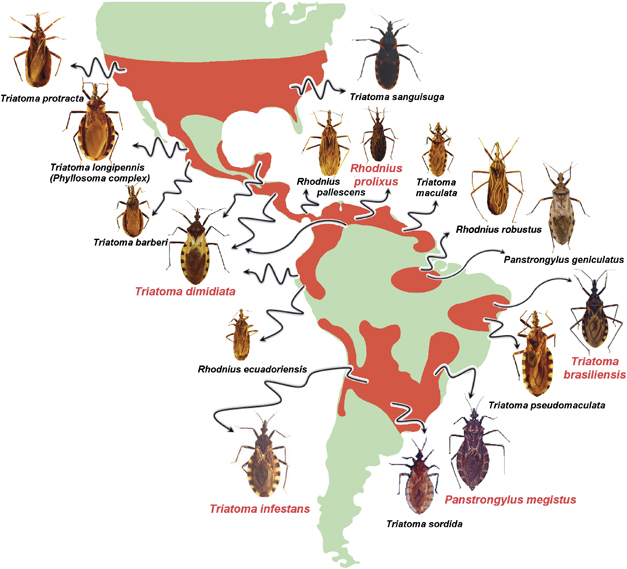
\includegraphics[scale=0.75]{slides/triatomine-map.jpg}
\end{frame}

%%%%%%%%%%%%%%%%%%%%%%%%%%%%%%%%%%%%%%%%%%%%%%%%%%%%%%%%%%%%%%%%%%%%%%%%%%%%%%%%%%%%%%%%%%%%%%%%%%%%%%%%%%%%
\begin{frame}{Chagas en Argentina y México}
	\begin{columns}

		\begin{column}{0.45\textwidth}
			\centering
				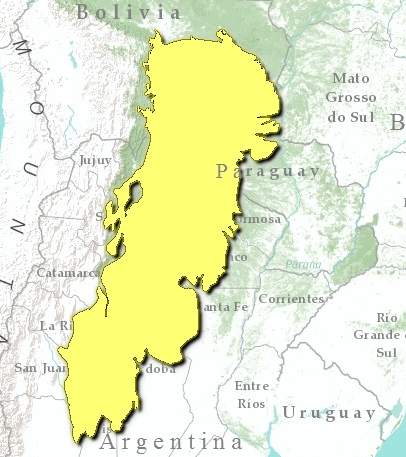
\includegraphics[height=.7\textheight]{slides/GranChaco_TNC-Argentina.jpeg}
		\end{column}
		% 	\medskip Las estimaciones de usuarios infectados oscilan alrededor de 1.5 millones de personas con solo 1 a 2 mil tratamientos realizados por año. En 2009 los tests de seroprevalencia en embarazadas alcanzaba el 4.2\% de casos.


		\begin{column}{0.45\textwidth}
			\centering
			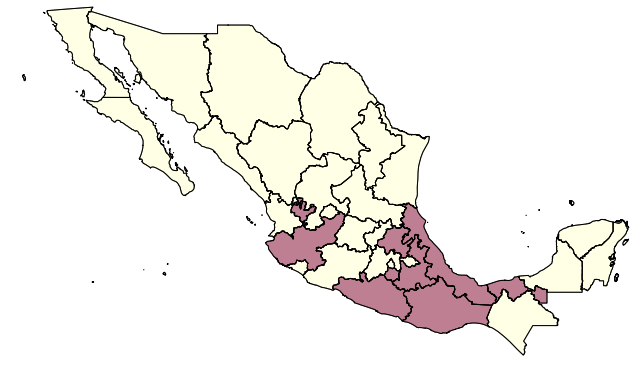
\includegraphics[width=\textwidth]{slides/Ambientes_Gran_Chaco-Mexico_original.png}
		\end{column}

% 			\medskip No oficialmente, los reportes estiman 5.5 millones de personas potencialmente afectados y donde menos del 0.5\% de los infectados tienen acceso a tratamientos

	\end{columns}
\end{frame}

% \begin{frame}{Puntos claves}
% 	% Chagas is a disease:
% 	El Chagas es una enfermedad:
% 	\begin{itemize}
% 		\item \ldots con diferentes vías de transmisión y donde las \textbf{migraciones de largo plazo} juegan un papel clave
% 		%explicar vertical, congenita y transfusion/transplante
% 		\item \ldots donde un pequeño número de la población infectada sabe que la está padeciendo
% 		% for which a low proportion of the infected population knows that they have the disease.
% 		\item \ldots con una fase asintomática que puede extenderse más de 10 años
% 		% % ORALLY SAY: 30 years of vector mitigation activities in GC.
% 		\item \ldots que es epidémica y desatendida
% 		% \item ... which is epidemic and unattended.
% 	\end{itemize}
% 	En particular, la fundación busca encontrar chagásicos en zonas no tradicionalmente endémicas
% 	%Es decir, gente de fuera de Gran Chaco infectada con \textit{Trypanosoma Cruzi} (el parásito que causa el Chagas).
% \end{frame}


%%%%%%%%%%%%%%%%%%%%%%%%%%%%%%%%%%%%%%%%%%%%%%%%%%%%%%%%%%%%%%%%%%%%%%%%%%%%%%%%%%%%%%%%%%%%%%%%%%%%%%%%%%%%%
\begin{frame}{Objetivo}
	\begin{block}{\ldots atacar esta problemática en América Latina}


	\begin{itemize}
		\item \ldots detectando \textbf{migraciones de largo plazo}
		\item \ldots utilizando datos de telefonía celular
		% for which a low proportion of the infected population knows that they have the disease.

		\item \ldots idealmente encontrando en fase asintomática
		% % ORALLY SAY: 30 years of vector mitigation activities in GC.
		% \item \ldots que es epidémica y desatendida
		% \item ... which is epidemic and unattended.
	\end{itemize}
	% Este trabajo propone un modelo que utiliza información de registros (logs) de llamados telefónicos
	% como forma de observar en qué regiones del país se espera encontrar una alta proporción de personas chagásicas

	% \bigskip
	% Sabiendo que las migraciones humanas tienen un rol crucial en la diseminación de la enfermedad, el modelo busca
	% detectar migraciones a partir de los patrones de uso celular
	% % , donde, idealmente, se vea que una fluida comunicación con el lugar de orígen es indicador
	\end{block}
\end{frame}

%%%%%%%%%%%%%%%%%%%%%%%%%%%%%%%%%%%%%%%%%%%%%%%%%%%%%%%%%%%%%%%%%%%%%%%%%%%%%%%%%%%%%%%%%%%%%%%%%%%%%%%%%%%%
\section{Clasificación Binaria Supervisada}
%%%%%%%%%%%%%%%%%%%%%%%%%%%%%%%%%%%%%%%%%%%%%%%%%%%%%%%%%%%%%%%%%%%%%%%%%%%%%%%%%%%%%%%%%%%%%%%%%%%%%%%%%%%%

\begin{frame}{Error de Predicción Esperado}
		\centering

		Sea $\textbf{X} \in \mathbb{R}^{n \times p}$ matriz aleatoria compuesta por muestras $\textbf{X}_i \in \mathbb{R}^{p}$\\
		$\textbf{Y} \in \mathbb{R}^n$ es el vector aleatorio de salida \\
		Se busca una función $f_\theta: \mathbb{R}^{p} \rightarrow  \mathbb{R}$ que optimice u ``aprenda''

	\begin{align*}%\label{expectedPredictionError}
		\begin{split}
		\operatorname{argmin}_{\theta} \  EPE(\theta) = & \Expect_{\textbf{X},\textbf{Y}} \left[ L(Y,f_\theta(X))\right]  \\
			= & \int L(y,f_\theta (x)) p(x,y) dx dy
		\end{split}
	\end{align*}

	para generar predicciones de \textit{cualquier} muestra

	\smallskip
	$f_\theta$ es un clasificador o algoritmo indexado por $\theta \in \Theta$

	\smallskip
	$L: \mathbb{R}^{2} \rightarrow  \mathbb{R}_{\geq 0}$ se denomina la función de pérdida


\end{frame}
%%%%%%%%%%%%%%%%%%%%%%%%%%%%%%%%%%%%%%%%%%%%%%%%%%%%%%%%%%%%%%%%%%%%%%%%%%%%%%%%%%%%%%%%%%%%%%%%%%%%%%%%%%%%

\begin{frame}{Consideraciones}

	$f_\theta^*$ intenta aproximar la relación desconocida entre $\textbf{X}$ y $\textbf{Y}$

	\bigskip

	$f(\cdot)$, $L(\cdot)$ y el espacio de búsqueda $\Theta$ de los \textit{aproximantes} son predeterminados

	\bigskip\

	Desconocemos $P(\textbf{X},\textbf{Y})$ pues nos basamos en datos finitos\\

	$X = \trainsetn  \sqcup \testsetn $

	\bigskip\
	En Clasificación: $y_i \in \{0,1\} \ \forall  i$ \ y \ $L(z,w) =  \mathbb{I}(z \neq w ) $

\end{frame}

%%%%%%%%%%%%%%%%%%%%%%%%%%%%%%%%%%%%%%%%%%%%%%%%%%%%%%%%%%%%%%%%%%%%%%%%%%%%%%%%%%%%%%%%%%%%%%%%%%%%%%%%%%%%

\begin{frame}{Aproximaciones de $EPE$}

Varios tipos de errores a minimizar en el aprendizaje con \textbf{finitos} datos observados
    \begin{block}{Error de entrenamiento y de generalización}

        $$  Err_{\trainsetn}(\theta) =
        \Expect_{ \textbf{X}, \textbf{Y} } \left[ L(Y,f_{\theta}(X))  |  \trainsetn \right] \approx
        \dfrac{1}{n} \sum_{i=1}^{n} \mathbb{I} \left(f_\theta (X_{i})\neq Y_{i} \right)  $$

        $$Err_{\testsetn}(\theta) \approx
        \dfrac{1}{n} \sum_{i=1}^{n} \mathbb{I} \left(f_\theta (\tilde{X_{i}})\neq \tilde{Y_{i}} \right)  $$

	\end{block}

	Un modelo se dice sobreajustado (``overfit'') cuando $\mid Err_{\testset}(\theta) - Err_{\trainset}(\theta)  \mid \ >> 0$

	Para esto es importante controlar la \textbf{complejidad} del modelo

\end{frame}

%%%%%%%%%%%%%%%%%%%%%%%%%%%%%%%%%%%%%%%%%%%%%%%%%%%%%%%%%%%%%%%%%%%%%%%%%%%%%%%%%%%%%%%%%%%%%%%%%%%%%%%%%%%%

\begin{frame}{ Ajuste Poly-M vs Ajuste Poly-2 }
\center\
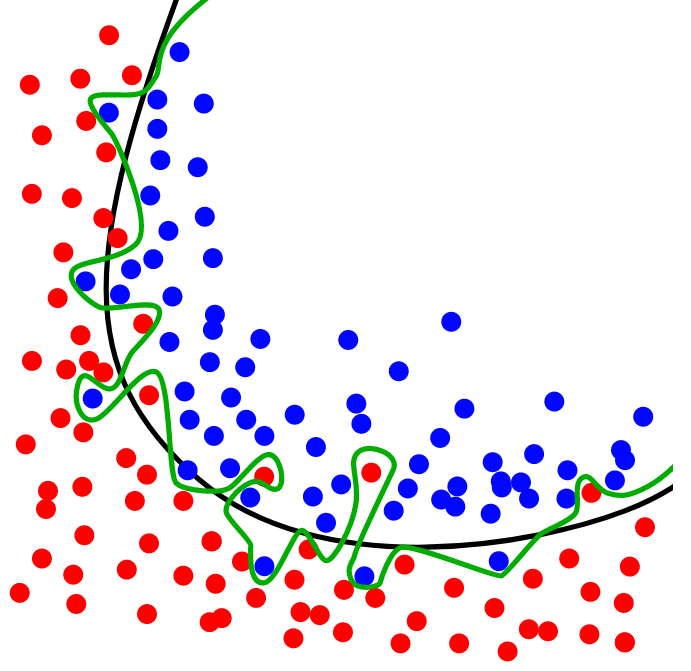
\includegraphics[width=0.9\textheight]{slides/wiki_overfit_complex_classifier_demo.png}
\end{frame}

%%%%%%%%%%%%%%%%%%%%%%%%%%%%%%%%%%%%%%%%%%%%%%%%%%%%%%%%%%%%%%%%%%%%%%%%%%%%%%%%%%%%%%%%%%%%%%%%%%%%%%%%%%%%

\begin{frame}{Convergencia a $EPE$ en clasificadores binarios}
Bajo ciertas condiciones sobre $\Theta$ tenemos
	\begin{block}{Desigualdad de Vapnik–Chervonenkis}

		\begin{align*}
			\begin{split}
				P\left(\sup_{\theta\in \Theta}\left|Err_{\trainsetn}(\theta)-EPE (\theta)\right|>\varepsilon \right) & \leq
				8S (\Theta,n) e^{{-n \varepsilon^{2}/32}}\\
				\Expect\left[\sup_{\theta \in \Theta}\left| Err_{\trainsetn}(\theta)-EPE (\theta)\right|\right] &
				\leq 2\sqrt{\dfrac{\log S(\Theta,n)+\log2}{n}}
			\end{split}
		\end{align*}
		
	\end{block}
	donde $S(\Theta)$ es el coeficiente de ``shattering'' de la clase
\end{frame}

%%%%%%%%%%%%%%%%%%%%%%%%%%%%%%%%%%%%%%%%%%%%%%%%%%%%%%%%%%%%%%%%%%%%%%%%%%%%%%%%%%%%%%%%%%%%%%%%%%%%%%%%%%%%

\begin{frame}[shrink=5]{Regresión Logística}

Con $\sigma(z) = \frac{1}{1 + e^{-z}}$ y $logodds(X_i)$ como $\log \left(  \frac{ P(C_1 \mid X_i)}{P(C_0 \mid X_i ) } \right)$
	\begin{block}{Idea}
	\footnotesize
		\begin{align*}
			P(C_1| X_i)  = \frac{1}{1 + \exp \left(- \log \left(  \frac{ P(X_i|C_1)p(C_1)}{P(X_i|C_0)p(C_0)} \right) \right)} = \sigma\left(logodds(X_i)\right)
		\end{align*}
	
		El modelo supone
		$$logodds(X_i) = \sum_{j=1}^p \theta^j \ X_i^j  \ , \forall X_i \in X $$
		$$Y_i \mid X_i \ \sim \operatorname{Bernoulli}(p_i)$$

	\end{block}

	\begin{block}{Función de pérdida (MLL)}
		$$\operatorname{argmin}_{\theta} \ \sum_{i=1}^N \big(Y_i ( \theta \cdot X_i ) + \log(1 + e^{1- \theta \cdot X_i} ) \big) + \lambda { \| \theta \|_{2}}^2$$
	\end{block}
	% $lambda$ es un hiperparámetro para la regularización del modelo
\end{frame}

%%%%%%%%%%%%%%%%%%%%%%%%%%%%%%%%%%%%%%%%%%%%%%%%%%%%%%%%%%%%%%%%%%%%%%%%%%%%%%%%%%%%%%%%%%%%%%%%%%%%%%%%%%%%

\begin{frame}[shrink=2]{Árbol de decisión}

Algoritmo recursivo y aleatorio que particiona el espacio en forma binaria $\mathcal{T}_{iz}(d,j) = \{x \in \mathcal{T} \ / \ x^j \leq d \}$ y $\mathcal{T}_{de}(d,j)$
		\begin{block}{Idea}
			% $$$
			\begin{align*}
				\min_{d, j} \big[ \min_{c_{iz} }  \frac{1}{N_{iz}}\sum_{x \in \mathcal{T}_{iz}(d,j) } Imp(y,c_{iz}) \
				+  \min_{c_{de}}  \frac{1}{N_{de}}\sum_{x \in \mathcal{T}_{de}(d,j) } Imp(y,c_{de}) \big]
			\end{align*}
				donde $Imp$ es una función de \textit{impureza}
			% \begin{align*}
			% \end{align*}
		\end{block}

		\begin{block}{Función de pérdida}
		\small
		{
		\center\
		$h_{\theta}(X_i) = \sum_{l=1}^L c_l I(X_i \in \mathcal{T}_l)$ \\
		}
	 	con $L$ el número de regiones. Aquí $\theta = \bigcup\limits_{l=1}^{L} (d_l,j_l)$
	
		\end{block}
\end{frame}

%%%%%%%%%%%%%%%%%%%%%%%%%%%%%%%%%%%%%%%%%%%%%%%%%%%%%%%%%%%%%%%%%%%%%%%%%%%%%%%%%%%%%%%%%%%%%%%%%%%%%%%%%%%%

\begin{frame}{Árbol de ejemplo}
		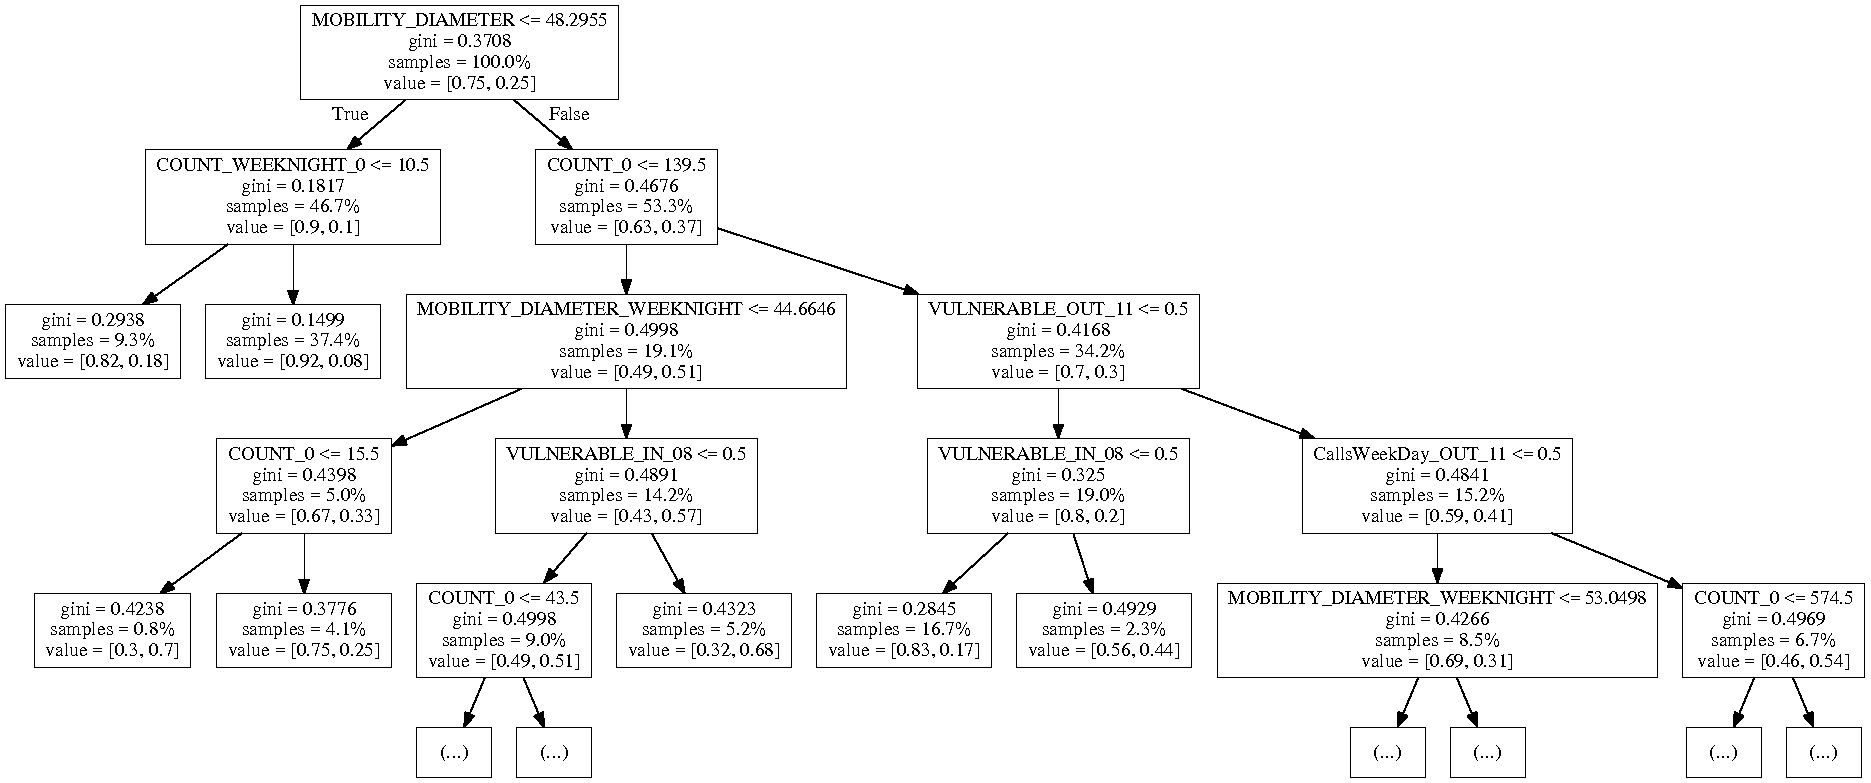
\includegraphics[width = 0.9 \paperwidth, height = 0.7 \paperheight,
										trim = 0.2 80 0.2 0.2cm, left, clip = true]{decision_tree/full_tree_map.png}
\end{frame}

%%%%%%%%%%%%%%%%%%%%%%%%%%%%%%%%%%%%%%%%%%%%%%%%%%%%%%%%%%%%%%%%%%%%%%%%%%%%%%%%%%%%%%%%%%%%%%%%%%%%%%%%%%%%

\begin{frame}{Sobreajuste con }
\center\
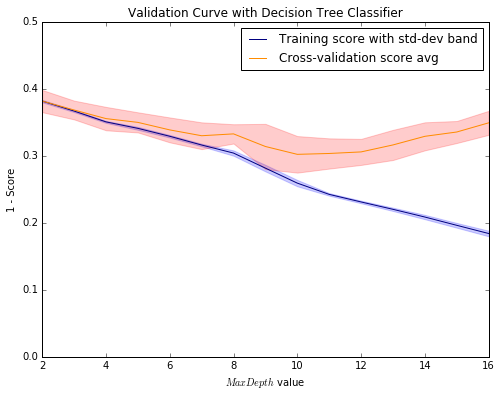
\includegraphics[width=1\textheight]{figure-biasVariance/dtree_overfit_problem_2.png}
\end{frame}

%%%%%%%%%%%%%%%%%%%%%%%%%%%%%%%%%%%%%%%%%%%%%%%%%%%%%%%%%%%%%%%%%%%%%%%%%%%%%%%%%%%%%%%%%%%%%%%%%%%%%%%%%%%%

\begin{frame}[shrink=2]{Clasificadores de Ensamble }

%	Sea $\bigcup\limits_{m=1}^{M} \{ h_{\theta_m} \}$ un conjunto de pequeños arboles

	\begin{block}{Bosques Aleatorios}
		\begin{align*}
			Y_i \approx f_{\theta}(X_i) = \dfrac{1}{M}\sum_{m=1}^M h_{\theta_m}(X_i)
		\end{align*}

	\end{block}

	\begin{block}{``Gradient Tree Boosting''}
		Mejora iterativa de la pérdida con pesos $\gamma$
		\begin{align*}
			f^{(M)}(X_i) = sgn \left(\sum_{m=1}^{M} \gamma_m h(X_i,\theta_m) \right)
		\end{align*}

		\begin{align*}
%			\begin{split}
				(\gamma_{m}, \theta_{m}) = \underset{\gamma, \theta}{\mathrm{argmin}} \sum_{i=1}^{N} & L\big( Y_i,  f^{m}(X_i) + \gamma h(X_i,\theta) \big)
%			\end{split}
		\end{align*}
		con \  $\theta^*_{m} = \underset{ \theta}{\mathrm{argmin}} \sum_{i=1}^{N}e^{-Y_i f^{m}(X_i)}
		\mathbb{I}\left[ Y_i \neq h(X_i,\theta)  \right]$ \ y \
		$\gamma^*_{m} = \frac{1}{2} \log\left( \frac{1 - Err(\theta^*) }{ Err(\theta^*) } \right)$

	\end{block}


\end{frame}


%%%%%%%%%%%%%%%%%%%%%%%%%%%%%%%%%%%%%%%%%%%%%%%%%%%%%%%%%%%%%%%%%%%%%%%%%%%%%%%%%%%%%%%%%%%%%%%%%%%%%%%%%%%%


\begin{frame}{``Naive Bayes''}

Suponemos una distribución conocida para $p(\cdot)$
	\begin{block}{Idea}
		Asumir \textit{inocentemente}
		$$p(X^j |X^1,\ldots,\overline{X^j},\ldots,X^p, C_k) \ = \ p(X^j | C_k) \ \forall k \in \{0,1\}$$
	\end{block}

	\begin{block}{Función de decisión }

		\begin{align*}
			p(C_1 \mid X) \propto f(X) = \hat{p}(C_{1}) \  \prod_{i=1}^{n} \hat{p}(X_{i}\mid C_{1})
		\end{align*}

		\begin{align*}
			\hat{Y} \ = \ \mathbb{I}\left[  f(X)  >= \ \frac{1}{2} \right]
		\end{align*}

	\end{block}
\end{frame}

%%%%%%%%%%%%%%%%%%%%%%%%%%%%%%%%%%%%%%%%%%%%%%%%%%%%%%%%%%%%%%%%%%%%%%%%%%%%%%%%%%%%%%%%%%%%%%%%%%%%%%%%%%%%

\begin{frame}{Estimación de Fronteras de Decisión}
		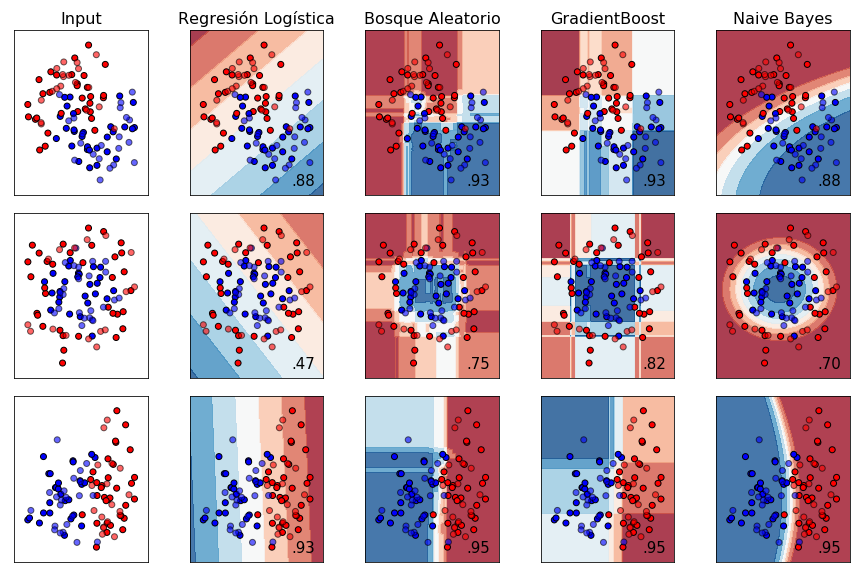
\includegraphics[width = 0.9 \paperwidth, height = 0.7 \paperheight,
										trim = 0.2 0.2 0.2 0.2cm, left, clip = true]{slides/plot_classifier_comparison.png}
\end{frame}

%%%%%%%%%%%%%%%%%%%%%%%%%%%%%%%%%%%%%%%%%%%%%%%%%%%%%%%%%%%%%%%%%%%%%%%%%%%%%%%%%%%%%%%%%%%%%%%%%%%%%%%%%%%%

\begin{frame}{$K$-Validación cruzada}

Optimización de configuraciones de hiperparámetros $\mathcal{A}$ vía estimación del $EPE$

	\begin{block}{Idea}
		Dado un $\alpha \in \mathcal{A}$, particionar las muestras en $K$ conjuntos al azar
		\\
		Entrenar $\hat{f}_{\alpha}^{-k}, \ k \in \{1, \ldots, K\}$
		\\
		donde cada clasificador $\hat{f}^{-k}$ se aprende sin las muestras de la partición $k$
		\\
		Computar $CV(\alpha) = \frac{1}{n} \sum^n_{i=1} L\left( y_i, \hat{f}_{\alpha}^{-k_i}(X_i) \right)$
	\end{block}

% un estimador insesgado del EPE, specially when K is high
% simple, convenient, analitico
% Similar a akaike IC (1 + 2x)
% no existe estimador insesgado de la varianza del K-CV

\end{frame}
%%%%%%%%%%%%%%%%%%%%%%%%%%%%%%%%%%%%%%%%%%%%%%%%%%%%%%%%%%%%%%%%%%%%%%%%%%%%%%%%%%%%%%%%%%%%%%%%%%%%%%%%%%%%

\begin{frame}{Métricas de clasificadores binarios}
	\center\
	Conteo de las combinaciones de $\hat{Y}$ y $Y$

		\begin{columns}
			\begin{column}{0.55 \textwidth}
			\scriptsize
				\noindent
				\renewcommand\arraystretch{1}
				\setlength\tabcolsep{0pt}
				\begin{tabular}{c >{\bfseries}r @{\hspace{0.7em}}c @{\hspace{0.4em}}c @{\hspace{0.7em}}l}
				\multirow{10}{*}{\parbox{1.1cm}{\bfseries\raggedleft\ Valor real $y$}} &
				& \multicolumn{2}{c}{\bfseries Valor predicho $\hat{y}$} & \\
				& & \bfseries \^{P} \ $(0)$ & \bfseries \^{N} \ $(1)$  \\
				& P \ $(0)$ & \MyBox{Verdadero}{Positivo (TP)} & \MyBox{Falso}{Negativo (FN)} & \\[2.4em]
				& N \ $(1)$ & \MyBox{Falso}{Positivo (FP)} & \MyBox{Verdadero}{Negativo (TN)} & \\
				%& total & P \ $(0)$ & &
				\end{tabular}

			\end{column}

			\begin{column}{0.45 \textwidth}
			\scriptsize
				\begin{align*}
					\begin{split}
						& Accuracy \ =\ \frac{ TP + TN }{ TP + TN + FP + FN }\\
						& Precision \ =\ \frac{ TP }{TP + FN}\\
						& Recall \  =\ \frac{TP }{TP + FP}\\
					  	& F1 = \mbox{media armónica de } Precision \mbox{ y } Recall \\
					  	& Curva \ ROC: \\
					  	& \sigma(\pi) = (Recall(\pi), FPR(\pi)) \ t.q. \ \pi \in (0,1)
					\end{split}
				\end{align*}
			\end{column}
		\end{columns}

	% \end{block}
\end{frame}



%%%%%%%%%%%%%%%%%%%%%%%%%%%%%%%%%%%%%%%%%%%%%%%%%%%%%%%%%%%%%%%%%%%%%%%%%%%%%%%%%%%%%%%%%%%%%%%%%%%%%%%%%%%%
\section{ Descripción de los datos}
%%%%%%%%%%%%%%%%%%%%%%%%%%%%%%%%%%%%%%%%%%%%%%%%%%%%%%%%%%%%%%%%%%%%%%%%%%%%%%%%%%%%%%%%%%%%%%%%%%%%%%%%%%%%

\begin{frame}{Visualización Social: El grafo de comunicaciones}
		\center\
		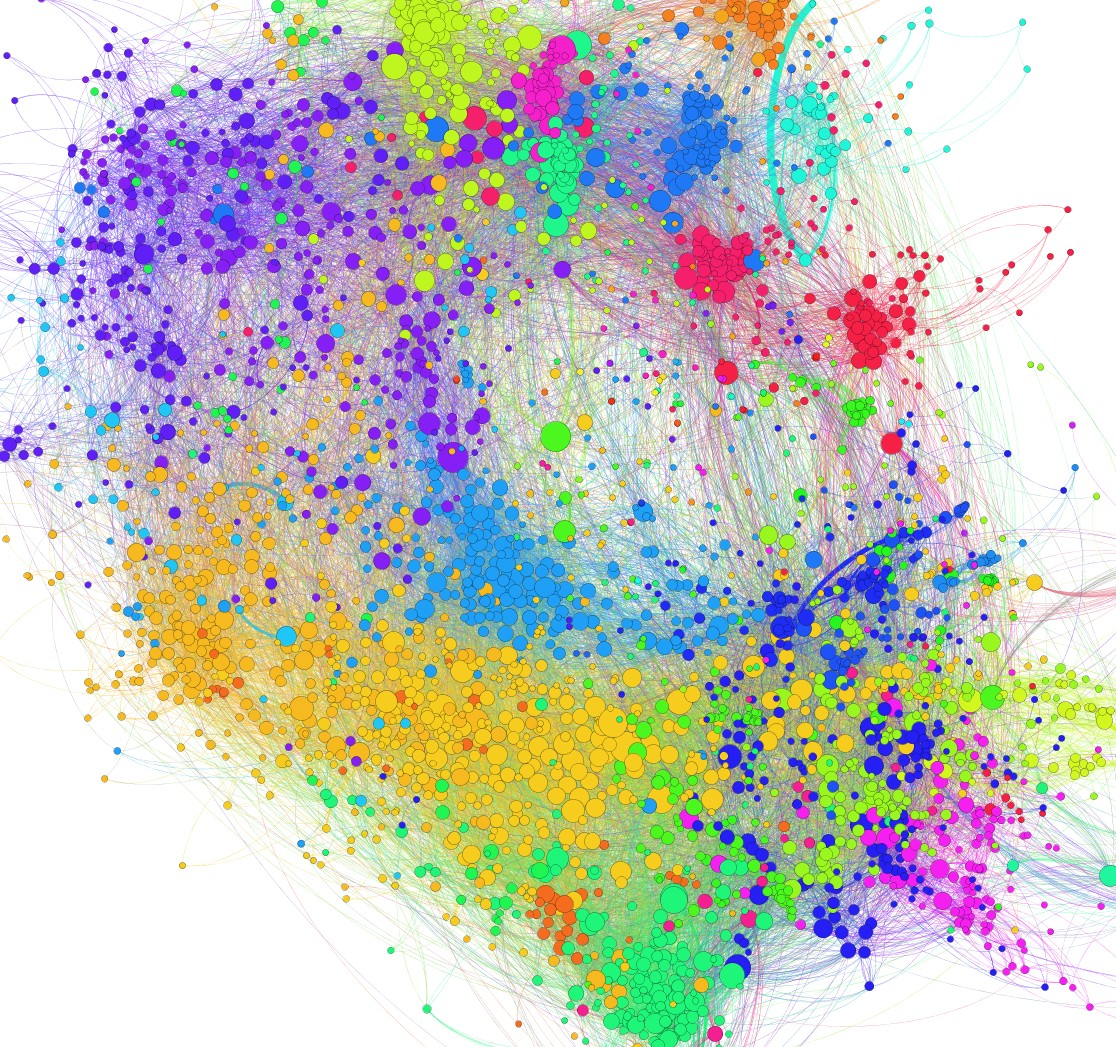
\includegraphics[scale=0.24]{slides/Graph-screenshot.jpg}
\end{frame}

%%%%%%%%%%%%%%%%%%%%%%%%%%%%%%%%%%%%%%%%%%%%%%%%%%%%%%%%%%%%%%%%%%%%%%%%%%%%%%%%%%%%%%%%%%%%%%%%%%%%%%%%%%%%
\begin{frame}{Registros de Llamados Celulares (CDRs)}

	$\approx$ 10 mil millones de registros detallados de llamados (CDRs) para México y Argentina con 24 y 5 meses de datos respectivamente.

	$$r =\left < u, w, t, d, a \right >$$
%	con
%	\begin{itemize}
%		\item Usuarios anonimizados $u$ y $w$ en esa llamada
%		\item Tiempo de inicio y duración de la llamada $t$
%		\item Dirección $d$ de la llamada (entrante o saliente, con respecto a $u$)
%		\item $a$ es el ID de la antena telefónica usada por $u$ en esa comunicación
%	\end{itemize}

	\medskip

 % realizados por 8 millones y 2 millones de usuarios, respectivamente para Argentina y México\footnote{No tenemos ninguna información personal de los usuarios como nombre, dirección, teléfono y su privacidad está asegurada mediante criptografía.}
% \medskip
% Para los dos países tenemos más de cuatro mil antenas celulares geolocalizadas

% \end{block}

	$H_u$ el lugar de residencia de un usuario y $E_z$ es el conjunto de antenas de la zona endémica
	\smallskip

	Tomamos dos períodos:
	\smallskip
	\begin{enumerate*}[label={\alph*)},]
			\item $T_0$ desde Enero 2014 hasta Julio 2015
			\item $T_1$ desde Agosto 2015 hasta Diciembre 2015
			% . Este va a ser nuestro dataset principal a procesar.
	\end{enumerate*}

	\medskip
	 $u$ es vulnerable si $\exists \ r = \ \left < u, w, t, d, a \right > $ tal que $H_w \in E_z$ para ese mes

	% que es determinado como la antena $a$ más utilizada de lunes a viernes y fuera del horario laboral. La endemicidad de un usuario está determinado por la condición $H_u \in E_Z$

\end{frame}

%%%%%%%%%%%%%%%%%%%%%%%%%%%%%%%%%%%%%%%%%%%%%%%%%%%%%%%%%%%%%%%%%%%%%%%%%%%%%%%%%%%%%%%%%%%%%%%%%%%%%%%%%%%%

% \begin{frame}{Agregación a nivel de antenas}

% 	%\pause\
% 	\begin{block}{Usuarios o llamados vulnerables}
% 	Para un mes dado y una antena $a$ tendremos la tupla $\left< N_a, V_a, C_a, VC_a \right>$ donde
% 		\begin{itemize}
% 			\item El número total de usuarios residentes $N_a$
% 			\item El número total de residentes vulnerables $V_a$
% 			\item El volumen total de llamados salientes $C_a$
% 			\item El volumen de llamados salientes en una interacción \textit{vulnerable} $VC_a$
% 		\end{itemize}
% 	% Esta  definen las propiedas are the properties we extracted for each antenna in the studied countries.
% 	\end{block}
% \end{frame}

%%%%%%%%%%%%%%%%%%%%%%%%%%%%%%%%%%%%%%%%%%%%%%%%%%%%%%%%%%%%%%%%%%%%%%%%%%%%%%%%%%%%%%%%%%%%%%%%%%%%%%%%%%%%
\begin{frame}
	\frametitle{Exploración con mapas de calor: Argentina $\geq$ = 1 \%}
	\center\
	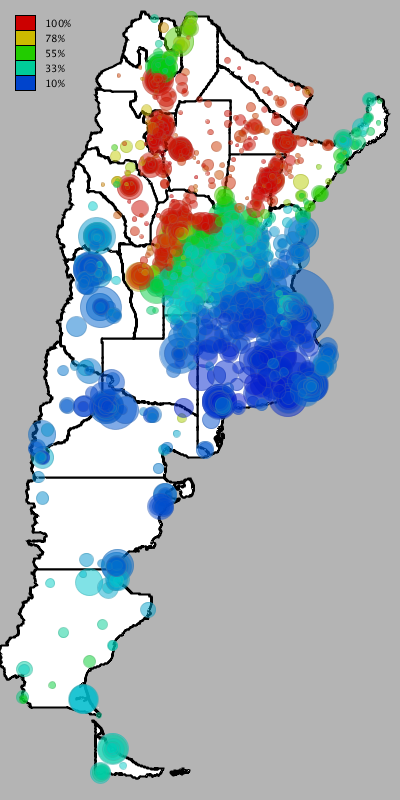
\includegraphics[height=.9\textheight,width = .9\columnwidth, keepaspectratio]
	{slides/201112_hi_res_argentina_usuarios_proporcion_circulos_beta1.png}
\end{frame}

%%%%%%%%%%%%%%%%%%%%%%%%%%%%%%%%%%%%%%%%%%%%%%%%%%%%%%%%%%%%%%%%%%%%%%%%%%%%%%%%%%%%%%%%%%%%%%%%%%%%%%%%%%%%
\begin{frame}
	\frametitle{Exploración con mapas de calor: Argentina, $\geq$ = 15 \%}
	\center\
	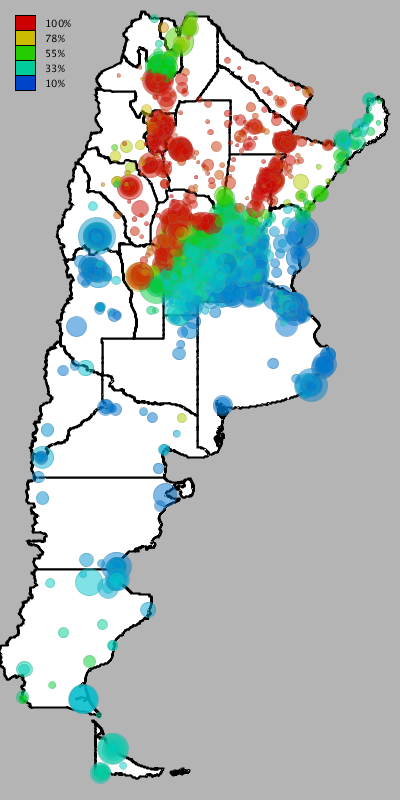
\includegraphics[height=.9\textheight,width = .9\columnwidth, keepaspectratio]
	{slides/201112_hi_res_argentina_usuarios_proporcion_circulos_beta15.png}
\end{frame}

%%%%%%%%%%%%%%%%%%%%%%%%%%%%%%%%%%%%%%%%%%%%%%%%%%%%%%%%%%%%%%%%%%%%%%%%%%%%%%%%%%%%%%%%%%%%%%%%%%%%%%%%%%%%
\begin{frame}
	\frametitle{Exploración con mapas de calor: Argentina, $\geq$ = 50 \%}
	\center\
	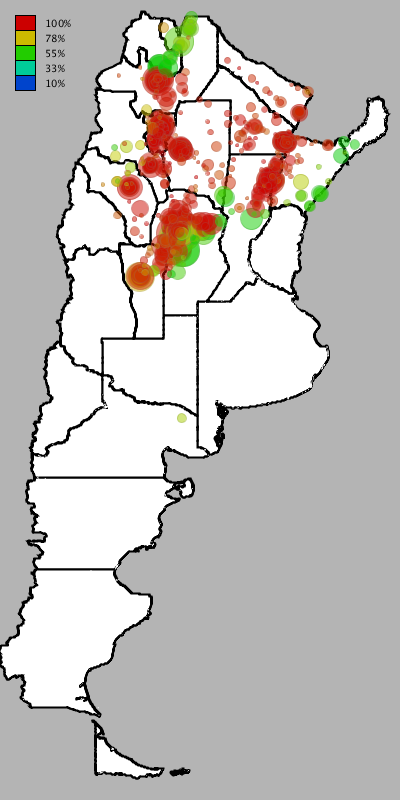
\includegraphics[height=.9\textheight,width = .9\columnwidth, keepaspectratio]
	{slides/201112_hi_res_argentina_usuarios_proporcion_circulos_beta50.png}
\end{frame}

%%%%%%%%%%%%%%%%%%%%%%%%%%%%%%%%%%%%%%%%%%%%%%%%%%%%%%%%%%%%%%%%%%%%%%%%%%%%%%%%%%%%%%%%%%%%%%%%%%%%%%%%%%%%
\begin{frame}
	\frametitle{Exploración con mapas de calor: AMBA, $\geq$ = 10 \%}
	\centering
	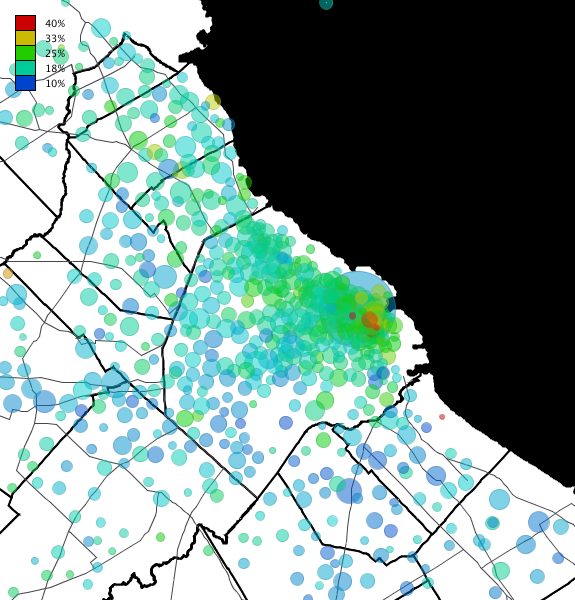
\includegraphics[height=.9\textheight,width = .9\columnwidth,keepaspectratio]
	{slides/201112_hi_res_amba_usuarios_proporcion_circulos_beta10.png}
\end{frame}
%%%%%%%%%%%%%%%%%%%%%%%%%%%%%%%%%%%%%%%%%%%%%%%%%%%%%%%%%%%%%%%%%%%%%%%%%%%%%%%%%%%%%%%%%%%%%%%%%%%%%%%%%%%%
\begin{frame}
	\frametitle{Exploración con mapas de calor: AMBA, $\geq$ = 20 \%}
	\centering
	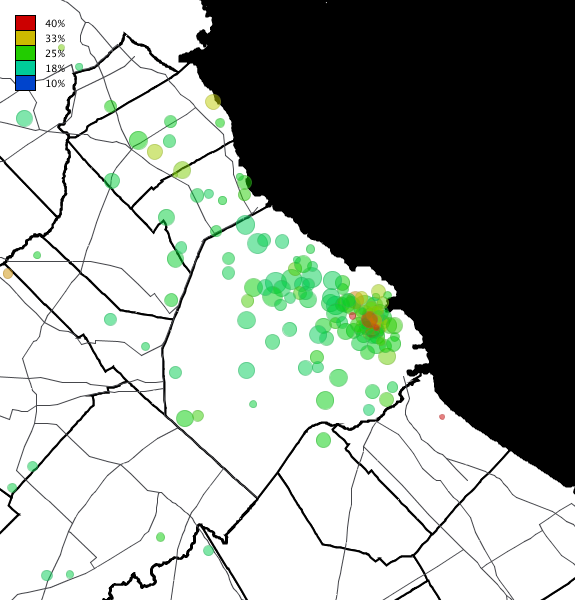
\includegraphics[height=.9\textheight,width = .9\columnwidth,keepaspectratio]
	{slides/201112_hi_res_amba_usuarios_proporcion_circulos_beta20.png}
\end{frame}
%%%%%%%%%%%%%%%%%%%%%%%%%%%%%%%%%%%%%%%%%%%%%%%%%%%%%%%%%%%%%%%%%%%%%%%%%%%%%%%%%%%%%%%%%%%%%%%%%%%%%%%%%%%%
\begin{frame}
	\frametitle{Exploración con mapas de calor, $\geq$ = 28 \%}
	\centering
	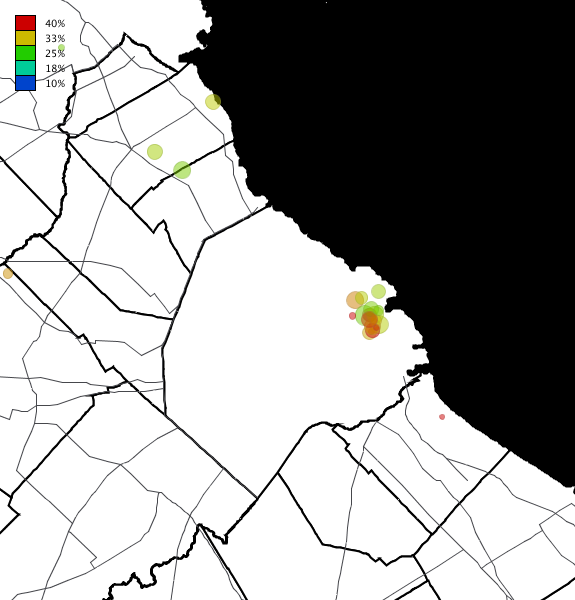
\includegraphics[height=.9\textheight,width = .9\columnwidth,keepaspectratio]
	{slides/201112_hi_res_amba_usuarios_proporcion_circulos_beta28.png}
\end{frame}

%%%%%%%%%%%%%%%%%%%%%%%%%%%%%%%%%%%%%%%%%%%%%%%%%%%%%%%%%%%%%%%%%%%%%%%%%%%%%%%%%%%%%%%%%%%%%%%%%%%%%%%%%%%%
%\begin{frame}{Comunidades vulnerables resaltadas}
%
%%	Luego de filtrar los mapas y explorar con distintas visualizaciones, encontramos antenas especificas que se resaltan por su nivel de vulnerabilidad
%	%Como resultado del filtrado en cada zona, nos hemos quedado con las antenas destacadas por su nivel de riesgo y, utilizando su ubicaci\'on, las emparejamos con localidades o comunidades argentinas.
%
%	\bigskip
%
%	\begin{block}{Comunidades relevantes en Argentina}
%		\begin{itemize}
%			\item Córdoba: Freyre, La Tordilla, Balnearia
%			%hay muchas mas pero no se si esta bien poner esto
%%			\item AMBA:\@ Avellaneda, Parque Patricios, San Isidro
%			\item Provincia de Buenos Aires: Lima, San Nicolás
%			\item La Rioja: Chamical y Malanzan
%			\item Salta: Tartagal
%		\end{itemize}
%
%	\end{block}
%\end{frame}


%%%%%%%%%%%%%%%%%%%%%%%%%%%%%%%%%%%%%%%%%%%%%%%%%%%%%%%%%%%%%%%%%%%%%%%%%%%%%%%%%%%%%%%%%%%%%%%%%%%%%%%%%%%%

\begin{frame}{Definición de problemas de migración A}

	$EU_{1}$ y $EU_{0}$ los conjuntos de usuarios que vivieron en la región endémica durante $T_1$ y $T_0$ respectivamente
	% así como también $H^0_u$ y $H^1_u$ para referirnos al hogar de $u$ a través de los períodos
	\begin{block}{Problema 1}
	Cuales usuarios vivían en la región endémica en el pasado:
		\begin{align*}
		Y^{(1)}_u =
		\begin{cases}
		&1 \ \mbox{if} \ u \in EU_{0} \\
		&0 \ \mbox{if not}.
		\end{cases}
		\end{align*}
	\end{block}


	\begin{block}{Problema 2}
		Cuales vivían en la región endémica y luego migraron:
		\begin{align*}
			Y^{(2)}_u =
			\begin{cases}
				&1 \ \mbox{if} \ u \in EU_{0} \cap { EU_{1} }^{\complement}  \\
				&0 \ \mbox{if not}.
			\end{cases}
		\end{align*}
	\end{block}

\end{frame}

%%%%%%%%%%%%%%%%%%%%%%%%%%%%%%%%%%%%%%%%%%%%%%%%%%%%%%%%%%%%%%%%%%%%%%%%%%%%%%%%%%%%%%%%%%%%%%%%%%%%%%%%%%%%

\begin{frame}{Definición de problemas de migración B}
	\begin{block}{Problemas 3}

		Predecir aquellos usuarios que migraron entre regiones, en cualquier dirección
		\begin{align*}
			Y^{(3)}_u =
			\begin{cases}
				&1 \ \mbox{if} \ u \in (EU_{0} \cap { EU_{1} }^{\complement}) \cup (EU_{1} \cap { EU_{0} }^{\complement}) \\
				&0 \ \mbox{if not}.
			\end{cases}
		\end{align*}
	\end{block}

	\begin{block}{Problema 4}
		Determinar, de todos los usuarios actualmente no endémicos, cuales migraron fuera de la región endémica
		\begin{align*}
			Y^{(4)}_u =
			\begin{cases}
				& 1 \ \mbox{if} \ u \in ( EU_{0} \cap { EU_{1} }^{\complement})    \\
				& 0 \ \mbox{if} \ u \in ( { EU_{1} }^{\complement} / EU_{0}).
			\end{cases}
		\end{align*}

	\end{block}

\end{frame}

%%%%%%%%%%%%%%%%%%%%%%%%%%%%%%%%%%%%%%%%%%%%%%%%%%%%%%%%%%%%%%%%%%%%%%%%%%%%%%%%%%%%%%%%%%%%%%%%%%%%%%%%%%%%

\begin{frame}{Atributos en los datos}
%	Solamente procesamos los CDRs de $T_1$
%	\bigskip

	\begin{block}{Diámetro de Movilidad}
		en kilómetros de la cápsula convexa generada por todas las antenas que un usuario utiliza en $T_1$. Hicimos la distinción para los registros de horarios no laborales.
	\end{block}

	\begin{block}{Región de residencia}
	Un usuario es asignado a una región a partir de $H_u$
\end{block}


	\begin{block}{Atributos del grafo de comunicaciones}
		En cada arista $\left< u, w \right>$ del grafo se desagrega la interacción en base a distintos criterios
		$\left< tiempo_{uw}, q\_llamados_{uw}, direccion, vulnerabilidad, momento, mes \right>$
%		donde $tiempo$ es el tiempo total en todos los llamados, $q\_llamados$ es la cantidad de llamados, $direccion$ es una variable booleana que indica si el llamado es entrante o saliente para $u$, $vulnerabilidad$ depende de si $w \in E_Z$ y $momento$ corresponde a una partición de la semana entre los días laborales, los fines de semana y los horarios no laborales
%
\end{block}


\end{frame}

%%%%%%%%%%%%%%%%%%%%%%%%%%%%%%%%%%%%%%%%%%%%%%%%%%%%%%%%%%%%%%%%%%%%%%%%%%%%%%%%%%%%%%%%%%%%%%%%%%%%%%%%%%%%
\begin{frame}{Ejemplo de atributos}
Un ejemplo de dos atributos de $X$ procesados a partir del grafo de comunicaciones
	\begin{table}[ht]
		\small
		\centering
		\resizebox{\textwidth}{!}{
			\begin{tabular} {|p{1.5cm}|p{1.5cm}|p{2cm}|p{1.5cm}|p{2cm}|p{1.5cm}|p{1cm}}
			% \begin{tabular} {|p{1.5cm} p{1.5cm} p{2cm} p{1.5cm} p{2cm} p{1.5cm} p{1cm}}
				%{l r r r r r r }
				% \toprule
				\toprule
				\textbf{Nombre del atributo} & \textbf{Q\_llamados / Tiempo} & \textbf{Momento} & \textbf{Dirección} &
				\textbf{Vulnerabilidad} & \textbf{Mes} \\
				% \midrule
				\midrule
				Llamados Fds EntrVul08    & Conteo & Final de Semana & Entrante & Interacciones vulnerables únicamente & Agosto\\
				% \midrule
				\midrule
				Tiempo LuVierNoche Sal12 & Tiempo de duración (s) & Durante la semana fuera de horario laboral & Saliente & Sin filtro endémico   & Diciembre \\
				% \hline
				\bottomrule
			\end{tabular}
		}
	\end{table}
\end{frame}


%%%%%%%%%%%%%%%%%%%%%%%%%%%%%%%%%%%%%%%%%%%%%%%%%%%%%%%%%%%%%%%%%%%%%%%%%%%%%%%%%%%%%%%%%%%%%%%%%%%%%%%%%%%%

\begin{frame}{ Proceso de experimentación }

Dado $(X,Y)$ y un algoritmo $\left( f, \Theta \right)  $
	\begin{enumerate}[I]
		% \item a
		% \item b
		\item Preprocesar $X$ y separar en $\trainset$ + $\testset$
		\item Cross validar hiperparámetros de $f$ c/ $\trainset$
		\item Aprender $f_\theta^*$ con $\trainset$
		\item Comparar  $Err_{\testset}(\theta^*)$ y  $Err_{\trainset}(\theta^*)$ en las métricas
		\item Evaluar ``best features'', mejoras en complejidad, e iterar en (I)
	\end{enumerate}

\end{frame}

\section{Resultados y Conclusiones}
%%%%%%%%%%%%%%%%%%%%%%%%%%%%%%%%%%%%%%%%%%%%%%%%%%%%%%%%%%%%%%%%%%%%%%%%%%%%%%%%%%%%%%%%%%%%%%%%%%%%%%%%%%%%


%%%%%%%%%%%%%%%%%%%%%%%%%%%%%%%%%%%%%%%%%%%%%%%%%%%%%%%%%%%%%%%%%%%%%%%%%%%%%%%%%%%%%%%%%%%%%%%%%%%%%%%%%%%%
\begin{frame}{Tabla de Experimentos A}

	\begin{table}[htp]\centering
	\footnotesize
		%\hskip-4.0cm
		\ra{1.3}
		%\hskip-4.0cm
		\begin{tabular}{@{}rr@{\hskip 0.3cm}r@{\hskip 0.3cm}r@{\hskip 0.3cm}rc@{}} \toprule
			&  \multicolumn{4}{c}{Problema 1} \\
			\cmidrule{2-5}
			& $Accuracy$ & $ROC AUC$ & $F1$ & $Runtime  (m)$ \\ \midrule
			$Regresion \ Logistica$     & 0.893 & 0.857 & 0.9   & 96\\
			$Bosques \ Aleatorios$            & 0.878 & 0.857 & 0.9  & 33 \\
			$GTB$ & 0.974 & 0.978 & 0.952 & 41  \\
			$Naive \ Bayes$               & 0.84  & 0.82  & 0.75  & 2  \\

			\bottomrule
		\end{tabular}

		%\addtocounter{table}{-1} % This dirty hack will fake both tables as if they were the same one.

		% \medskip
		%\hskip-4.0cm
		\ra{1.3}
		%\hskip-4.0cm
		\begin{tabular}{@{}rr@{\hskip 0.3cm}r@{\hskip 0.3cm}r@{\hskip 0.3cm}rc@{}} \toprule
			&  \multicolumn{4}{c}{Problema 2} \\
			\cmidrule{2-5}
			& $Accuracy$ & $ROC AUC$ & $F1$ & $Runtime  (m)$ \\ \midrule
			$Regresion \ Logistica$     & 0.714 & 0.726 & 0.248 & 119 \\
			$Bosques \ Aleatorios$            & 0.79  & 0.776 & 0.278 & 45  \\
			$GTB$ & 0.838 & 0.819 & 0.291 & 54 \\
			$Naive \ Bayes$               & 0.64  & 0.61  & 0.31  & 2   \\

			\bottomrule
		\end{tabular}
	\end{table}

\end{frame}


\begin{frame}{Tabla de Experimentos B}

	\begin{table}[htp]\centering
	\footnotesize
		\ra{1.3}
		%\hskip-4.0cm
		\begin{tabular}{@{}rr@{\hskip 0.3cm}r@{\hskip 0.3cm}r@{\hskip 0.3cm}rc@{}} \toprule
			&  \multicolumn{4}{c}{Problema 3} \\
			\cmidrule{2-5}
			& $Accuracy$ & $ROC AUC$ & $F1$ & $Runtime  (m)$ \\ \midrule
			$Regresion \ Logistica$     & 0.705 & 0.754 & 0.307 & 115 \\
			$Bosques \ Aleatorios$            &  0.792 & 0.845 & 0.346 & 21 \\
			$GTB$ & 0.811 & 0.855 & 0.359 & 33 \\
			$Naive \ Bayes$               & 0.65  & 0.63  & 0.45  & 1  \\

			\bottomrule
		\end{tabular}
		%\hskip-4.0cm
		% \medskip
		\ra{1.3}
		%\hskip-4.0cm
		\begin{tabular}{@{}rr@{\hskip 0.3cm}r@{\hskip 0.3cm}r@{\hskip 0.3cm}rc@{}} \toprule
			&  \multicolumn{4}{c}{Problema 4} \\
			\cmidrule{2-5}
			& $Accuracy$ & $ROC AUC$ & $F1$ & $Runtime  (m)$ \\ \midrule
			$Regresion \ Logistica$     & 0.883 & 0.85  & 0.331 & 106 \\
			$Bosques \ Aleatorios$            & 0.898 & 0.853 & 0.393 & 19 \\
			$GTB$ & 0.885 & 0.873 & 0.384 & 47 \\
			$Naive \ Bayes$               & 0.85  & 0.76  & 0.62 & 1 \\

			\bottomrule
		\end{tabular}
	\end{table}

\end{frame}



\begin{frame}{Resultados}

	\begin{block}{ Problema 1 Correlacionado}
		Todas las métricas $\geq 75\%$ con la mejor en $97\%$
	\end{block}

	\begin{block}{Muy bajo $F1$}
		\begin{itemize}[]
			\item Desbalance de clases deriva en sobre-confianza
			\item Precision y ``Recall'' asimétricos
			\item Sorpresa en ``Naive Bayes'' para ser hasta $50\%$ mejor en el Problema 4
			\item El Problema 2 es de mayor desbalance
		\end{itemize}
	\end{block}

\begin{block}{Inconvenientes en la ``Regresión Logística''}
	\begin{enumerate}[I]
		\item Lento: 110 min promedio frente a 1 min para ``Naive Bayes''
		\item Hasta un $12\%$ peor que $GBT$
	\end{enumerate}
\end{block}

\end{frame}

%%%%%%%%%%%%%%%%%%%%%%%%%%%%%%%%%%%%%%%%%%%%%%%%%%%%%%%%%%%%%%%%%%%%%%%%%%%%%%%%%%%%%%%%%%%%%%%%%%%%%%%%%%%%

\begin{frame}{Mejores Atributos}

		Heurística para algoritmos de ensamble

		\begin{itemize}
			\item Interacciones en el mes de Diciembre o en Agosto
			\item Interacciones vulnerables
			\item Diámetro de Movilidad
		\end{itemize}

\end{frame}

%%%%%%%%%%%%%%%%%%%%%%%%%%%%%%%%%%%%%%%%%%%%%%%%%%%%%%%%%%%%%%%%%%%%%%%%%%%%%%%%%%%%%%%%%%%%%%%%%%%%%%%%%%%%

\begin{frame}{Conclusiones Esperadas}

	Descenso de temperatura desde el ``Gran Chaco'' hacia afuera
	% , indicando que las antenas descienden su porcentaje de usuarios \textit{vulnerables}

	\medskip
	Las interacciones vulnerables eran atributos relevantes
	% de llamados desde y hacia la región endémica son relevantes para predecir migraciones
	% , lo cual confirma nuestra hipótesis utilizada para construir los mapas de calor

	\medskip
	% Fue posible construir clasificadores de
	Alta performance en $Accuracy$ y $ROC AUC$ 	++ ensamble
	% para detectar cuáles usuarios migraron desde la región endémica
	% , sobre todos los usuarios actualmente no endémico

	\medskip

	Utilización novedosa de los CDRs
	% es novedosa de los CDRs y se puede extender hacia otras epidemias

\end{frame}

%%%%%%%%%%%%%%%%%%%%%%%%%%%%%%%%%%%%%%%%%%%%%%%%%%%%%%%%%%%%%%%%%%%%%%%%%%%%%%%%%%%%%%%%%%%%%%%%%%%%%%%%%%%%
%%%%%%%%%%%%%%%%%

\begin{frame}{Conclusiones Inesperadas}

	\begin{itemize}[]
		\item Mapas correlacionan con migraciones
		\item $--$ precisión y $F1$ en general
		\item Los meses también fueron atributos relevantes

	\end{itemize}
\end{frame}

%%%%%%%%%%%%%%%%%%%%%%%%%%%%%%%%%%%%%%%%%%%%%%%%%%%%%%%%%%%%%%%%%%%%%%%%%%%%%%%%%%%%%%%%%%%%%%%%%%%%%%%%%%%%
%%%%%%%%%%%%%%%%%

% \begin{frame}{Inconvenientes}

% 		\begin{block}{Sesgos en los datos}
% 			\begin{itemize}
% 			\item Basados únicamente en datos de una sola TelCo por país que no capturan migraciones internacionales
% 			%La caracterizaci\'on actual de la vulnerabilidad viene dada por contacto telefónicos con usuarios de antenas del Gran Chaco.
% 			\item Concentración geoespacial de usuarios

% 			\item Mobilidad no implica prevalencia

% 			\item Estacionalidades en las migraciones

% 			\end{itemize}
%  	 	\end{block}
% \end{frame}


  %%%%%%%%%%%%%%%%%%%%%%%%%%%%%%%%%%%%%%%%%%%%%%%%%%%%%%%%%%%%%%%%%%%%%%%%%%%%%%%%%%%%%%%%%%%%%%%%%%%%%%%%%%%%

% \begin{frame}{Lineas Futuras de Trabajo}
%
%	\begin{block}{Extensiones}
%
%		\begin{enumerate}[I]
%			\item + clasificadores
%			\item Metodos para desbalance
%			\item + ``best features''
%			\item Feature Engineering
%			\item Estacionaridad
%			\item datos de serologia u ruralidad
%		\end{enumerate}
%
%	\end{block}
%% 	\medskip
%% 	\begin{block}{Nuevas fuentes de datos}
%% 		Agreagar informacion para mayores analisis:
%% 		\begin{itemize}
%% 			\item estimación de resultados de movilidad con serologia por region
%% 			\item Categorizacion de antenas por grado de ruralidad del ambiente
%% 			\item infected newborns
%% 			\item acute Chagas cases.
%% 			\item serological data per community, amongst others.
%% 		\end{itemize}
%% 	\end{block}
%
% \end{frame}

%%%%%%%%%%%%%%%%%%%%%%%%%%%%%%%%%%%%%%%%%%%%%%%%%%%%%%%%%%%%%%%%%%%%%%%%%%%%%%%%%%%%%%%%%%%%%%%%%%%%%%%%%%%%
% ==============================================

\begin{frame}{Gracias! }

	\begin{block}{Compañeros de proyecto}
					\center\
					Carolina Lang (UBA, GranData Labs) \\
					 Diego Weinberg (Fundación Mundo Sano) \\
	\end{block}

		% \begin{column}{0.55 \textwidth}
				\center\
				Juan Mateo de Monasterio \\
				\textit{laterio@gmail.com} \\
				Preguntas? \\
		% \end{column}

\end{frame}



% ==============================================

\justifying%
\scalefont{0.7}
% \bibliographystyle{unsrtnat}
% \bibliography{./}

% \end{columns}
% ==============================================

\vfill

\end{document}